% Proposta (12/11/2026, pedido do autor): linha do tempo só com os períodos de
% teste, para a seção 2.2 (amostra), antes da Figura 7, que acrescenta a
% otimização. Mesma escala e mesmo estilo da fig07-periodos.tex, sem as barras
% de otimização. Eixo a partir de 2006 (sem a otimização, 2004 a 2006 ficaria
% vazio) e rótulos com as palavras da 2.2. Fora do TG até o autor decidir.
% Procedência das datas (as mesmas da fig07):
%   2007 a 2011, 2013 a 2016 e 2025 a 2026: tabela do
%     dados/resultados/refeito_2026-10-05/PROTOCOLO.md (T1, T2, T3);
%   2017 a 2024: primeira e última linha de
%     dados/resultados/refeito_2026-10-05/testes/curva_R6_GS.csv
%     (2017-01-02 e 2024-12-27);
%   faixas de 2008 e 2020: anos-calendário dos recortes do Cap. III.
\documentclass[10pt,border=2pt]{standalone}
\usepackage[T1]{fontenc}
\usepackage[utf8]{inputenc}
\usepackage{mathptmx}
\usepackage{tikz}
% posição horizontal de uma data: 0,6 cm por ano a partir de 01/01/2006
\newcommand{\X}[3]{\fpeval{0.6*((#1-2006) + (#2-1)/12 + (#3-1)/365)}}
\tikzset{
  teste/.style={draw, semithick, fill=gray!12, minimum height=5mm},
  txt/.style={font=\footnotesize, inner sep=1pt},
}
% \barra{linha}{a1}{m1}{d1}{a2}{m2}{d2}{texto}
\newcommand{\barra}[8]{%
  \filldraw[teste] (\X{#2}{#3}{#4}, #1-0.25) rectangle (\X{#5}{#6}{#7}, #1+0.25);
  \node[txt] at ({(\X{#2}{#3}{#4}+\X{#5}{#6}{#7})/2}, #1) {#8};}
\begin{document}
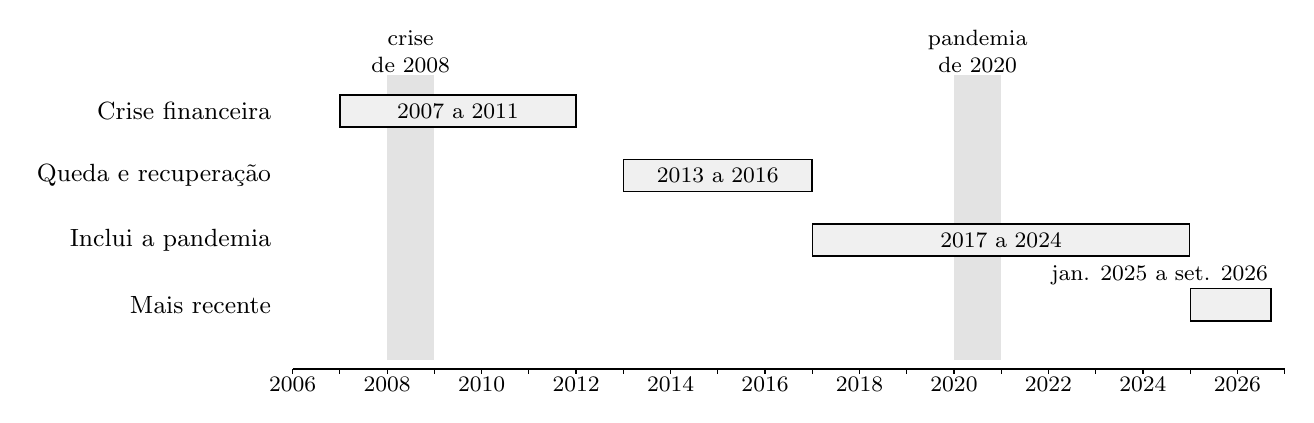
\begin{tikzpicture}[y=0.82cm]
  \fill[gray!22] (\X{2008}{1}{1}, -3.85) rectangle (\X{2009}{1}{1}, 0.55);
  \fill[gray!22] (\X{2020}{1}{1}, -3.85) rectangle (\X{2021}{1}{1}, 0.55);
  \node[txt, above, align=center] at ({\X{2008}{7}{1}}, 0.55) {crise\\de 2008};
  \node[txt, above, align=center] at ({\X{2020}{7}{1}}, 0.55) {pandemia\\de 2020};

  \foreach \y/\r in {0/{Crise financeira}, -1/{Queda e recuperação}, -2/{Inclui a pandemia},
                     -3/{Mais recente}}
    \node[anchor=east, font=\small] at (-0.15, \y) {\r};

  \barra{0}{2007}{1}{2}{2011}{12}{30}{2007 a 2011}
  \barra{-1}{2013}{1}{2}{2016}{12}{30}{2013 a 2016}
  \barra{-2}{2017}{1}{2}{2024}{12}{27}{2017 a 2024}
  \barra{-3}{2025}{1}{2}{2026}{9}{18}{}
  \node[txt, anchor=south east] at ({\X{2026}{9}{18}}, -2.75) {jan. 2025 a set. 2026};

  \draw[semithick] (0, -4) -- (\X{2027}{1}{1}, -4);
  \foreach \a in {2006,...,2027} \draw (\X{\a}{1}{1}, -4) -- ++(0, -0.08);
  \foreach \a in {2006,2008,...,2026}
    \node[txt, below] at (\X{\a}{1}{1}, -4.08) {\a};
\end{tikzpicture}
\end{document}
